\documentclass[a4,12pt]{article}

%\usepackage{showframe}
\usepackage{fontspec}
\setmainfont[Path = ./fonts/,
BoldFont={MinionPro-Bold.otf},
ItalicFont={MinionPro-It.otf}
]{MinionPro-Regular.otf}
\usepackage{amsmath,amssymb}
\usepackage{graphicx}
\graphicspath{ {./images/} }
\usepackage{hyperref}
\hypersetup{
    colorlinks=true,
    linkcolor=black,
    urlcolor=black,
    citecolor=black,
}
\usepackage[round]{natbib}
\bibliographystyle{plainnat}
\usepackage{bibentry}
\usepackage{url}
\usepackage[normalem]{ulem}
\usepackage{xcolor}
\usepackage{setspace}
\usepackage{multirow}
\usepackage{enumitem}
\usepackage{./peripheral/tuebingerspruechle-utf8}
\usepackage{tocloft}
\usepackage[nottoc]{tocbibind}
\renewcommand{\bibname}{References}
\renewcommand{\cftsecleader}{\cftdotfill{\cftdotsep}}
\usepackage{booktabs}
\usepackage{tikz}
\usepackage{tabularx}
\usepackage{tikz-qtree}
\usepackage{pdflscape}
\usepackage{float}
\usepackage{caption}
\usepackage{subcaption}
\usepackage{gb4e}

\newcolumntype{L}[1]{>{\raggedright\arraybackslash}p{#1}}
\newcolumntype{C}[1]{>{\centering\arraybackslash}p{#1}}
\newcolumntype{R}[1]{>{\raggedleft\arraybackslash}p{#1}}

\onehalfspacing

\title{Analyzing Linguistic Complexity of L2 Portuguese for Automatic Proficiency Classification}
\author{Eric DeMattos}
\date{July 2020}

\begin{document}

%%%%%%%%%%%%%%%%%%%%%%%%%%%%%%%%%%%% front matter

\pagenumbering{roman}

\thispagestyle{empty} % remove page number

\begin{center}
\noindent
\vspace{\fill}

Eberhard Karls Universität Tübingen\\
Seminar für Sprachwissenschaft

\vspace{\fill}


\hrule
\vspace{1em}
{\Large Analyzing Linguistic Complexity of {\scshape l2} Portuguese \\
\vspace{0.25em}
for Automatic Proficiency Classification}
\vspace{1em}
\hrule

\vspace{\fill}

\begin{flushleft}
{\scshape author} \hfill {\scshape advisor}\\
Eric DeMattos \hfill Prof. Dr. Detmar Meurers
\end{flushleft}

\vspace{\fill}

August 2020

\end{center}

\clearpage


\SpruechleAufsagen{Eric DeMattos} 

\begin{picture}(10,5)
\put(60,25){\includegraphics[scale=0.12]{signature1.png}}
\end{picture}

\clearpage

\begin{abstract}
    
This thesis explores the interaction between different linguistic complexity features and their efficacy in automatically classifying proficiency levels in {\scshape l2} Portuguese learners using supervised machine learning. We have found that even a small subset of complexity measures are useful, though supplementing them with other information may lead to further improvements. This analysis also corroborates previous findings in second language acquisition research that has posited various complexity features as good indicators of language growth.

\end{abstract}
\pagebreak
\tableofcontents
\pagebreak

%%%%%%%%%%%%%%%%%%%%%%%%%%%%%%%%%%%% body

\pagenumbering{arabic}
\section{Introduction}

Automated essay scoring has received increased attention in recent years due to the mainstream adoption of digital education platforms and the proliferation of annotated corpora on which to evaluate such systems. One emerging application of this field is automatic proficiency classification: assessing language learner text and mapping their level on a scale, e.g.\ the Common European Framework of Reference for Languages (CEFR). For a time, research had mostly centered around English, though efforts have been made to expand the landscape to other languages such as German \citep{hancke2013-german, weiss2019-german}, Swedish \citep{ostling2013-swedish, pilan2016-swedish}, Estonian \citep{vajjala2014-estonian}, Norwegian \citep{berggren2019-norwegian}, Spanish \citep{delrio2019b}, and even cross-lingually for German, Czech, and Italian \citep{vajjala2018-cefr}.

Following the introduction of a Portuguese learner corpus \citep{delrio2018}, the first automatic proficiency classification tests for the ``language of Camões" have surfaced \citep{delrio2019a, delrio2019b}. In these studies, del Río initially experimented with bag-of-words, POS and dependency \textit{n}-grams, and a modest amount of linguistic complexity features, obtaining 72\% accuracy with bag-of-words and POS \textit{n}-grams being the best performing features. She later investigated cross-lingual Spanish-Portuguese classification in view of their morphosyntactic proximity, but did not surpass the results of her previous work.

Since linguistic complexity has been identified as one of the core dimensions characterizing language proficiency \citep{housen2009}, one would expect it to be a well-suited metric for measuring growth. The lack of resources available in this area for Iberian languages, however, has heretofore impeded further research. In response, this thesis aims to expand support for extracting complexity features of European Portuguese and explore a larger set of feature interactions to determine whether it can indeed be a better indicator of language proficiency. To that end, it will provide a new platform on which to calculate such measures for Portuguese in a multilingual context.


\section{Background}

\subsection{Portuguese}
\label{section:pt}

Portuguese is the mother tongue of approximately 215 million people globally, making it the sixth most spoken in the world by number of native speakers. It is the official language of seven countries and maintains co-official status in three others. The language is further divided into two main dialects that are generally mutually intelligible: European and Brazilian. The varieties of Lusophone countries in Africa and Asia often resemble their European counterpart more closely due to prolonged colonial rule, though the influence of indigenous languages and the transatlantic slave trade resulted in some shared phonological and prosodic divergence among certain African variants and Brazilian Portuguese in particular.

Similar to other Romance languages, Portuguese is characterized by moderate fusional inflection and, by consequence, a somewhat less rigid word order. While it is generally an SVO language, it also allows for SOV constructs when, for example, object pronouns are realized preverbally in what is known as proclisis. Object pronouns may otherwise be attached after the verb as an enclitic, with usage varying by dialect and context. There also exists a mesoclitic construction—restricted to verbs in the future or conditional tense—wherein a personal pronoun, object pronoun, or both may be inserted between a verb stem and its inflectional suffix.

\begin{exe}
\ex\label{pro}
\gll me\ chamo\\
{\scshape 1.sg}=call.{\scshape 1.sg.pres}\\
\glt ``(I) call myself" \citep{galves2005}

\ex\label{en}
\gll chamo-me\\
call.{\scshape 1.sg.pres}={\scshape 1.sg}\\
\glt ``(I) call myself" \citep{galves2005}

\ex\label{meso}
\gll dar-lhes-ão\\
give={\scshape dat.3.pl=3.pl.fut}\\
\glt ``(they) will give them" \citep{wetzels2018}
\end{exe}

Contractions are also ubiquitous in both written and spoken Portuguese, irrespective of register. Many common function word pairs are realized exclusively in their merged forms, analogous to French \textit{du} (de + le) and Spanish \textit{al} (a + el). A few examples of mandatorily-contracted words are provided in Table~\ref{tab:contractions}.

\begin{table}[ht]
\renewcommand{\arraystretch}{1.2}
    \centering
    \begin{tabular}{@{}c|cccc@{}}
         & \textit{o} & \textit{a} & \textit{os} & \textit{as} \\
        \hline
        \textit{a} & \textit{ao} & \textit{à} & \textit{aos} & \textit{às} \\
        \textit{de} & \textit{do} & \textit{da} & \textit{dos} & \textit{das} \\
        \textit{em} & \textit{no} & \textit{na} & \textit{nos} & \textit{nas} \\
        \textit{por} & \textit{pelo} & \textit{pela} & \textit{pelos} & \textit{pelas} \\
    \end{tabular}
    \caption{Subset of prepositions merging with definite articles marked for gender and number. From top to bottom: to, from, in, for.}
    \label{tab:contractions}
\end{table}

Portuguese, similar to other languages, contains multiple cleft constructions used to bring a constituent into focus. There are five main variants according to \cite{lobo2019} that are acquired at different stages of linguistic development, including the atomic \textit{é que} cleft illustrated in (\ref{eque}).

\begin{exe}
\ex\label{eque}
\gll Este ator é que a Academia escolheu.\\
this actor be.{\scshape pres} that the Academy choose.{\scshape past}\\
\glt ``It was this actor that the Academy chose." \citep{lobo2019}
\end{exe}

Another characteristic of Portuguese is the presence of an infinitive inflection, allowing for person and number agreement with an overt or implicit subject in embedded contexts without a subordinating conjunction \citep{inf, inflinf}. The distinction is exemplified in (\ref{inflinf1}-\ref{inflinf2}) with the verb \textit{ir} ``to go".

\begin{exe}
\ex\label{inflinf1}
\gll Lamento que tu não vás à festa \\
{(I) regret} that you not go.{\scshape 2.sg.subj} to.the party \\
\glt ``I regret that you don’t go to the party." \citep{inflinf}

\ex\label{inflinf2}
\gll Lamento tu não ires à festa \\
{(I) regret} you not go.{\scshape 2.sg.inf} to.the party. \\
\glt ``I regret that you haven’t gone to the party." \citep{inflinf}
\end{exe}

These features will be further discussed in Section~\ref{section:discussion} in relation to their efficacy in proficiency classification.

%%%%%%%%%%%%%%%%%%%%%%%%%%%%%%%%%%%%%%
%%%%%%%%%%%%%%%%%%%%%%%%%%%%%%%%%%%%%%
%%%%%%%%%%%%%%%%%%%%%%%%%%%%%%%%%%%%%%

\subsection{Automatic Proficiency Classification}

\defcitealias{cefr2001}{Council of Europe, 2001}

Students learning a language are often categorized according to their skill level to determine their different abilities and needs. Various standards exist for assessing this, though one of the most popular is the Common European Framework of Reference for Languages \citepalias[CEFR;][]{cefr2001}. Three coarse reference levels ranging from A (basic) to C (proficient) are used to delineate broad groups of students, each of which can be further divided into two sublevels: A1 (beginner), A2 (elementary), B1 (intermediate), B2 (upper intermediate), C1 (advanced), and C2 (mastery).

An empirical scale on which to measure proficiency is useful for identifying materials suitable for a student's level that will challenge them appropriately and foster growth. Comprehensible input is requisite for learners to build on concepts they already understand while exploring new aspects of the language \citep[$i+\text{1}$;][]{krashen1981}. For this reason, it is crucial to place students at the appropriate level so that they are not under-stimulated, though not so high that they are pushed beyond their Zone of Proximal Development—the space in which they are able to perform tasks successfully, with or without assistance \citep{vygotsky1986}.

With the burgeoning availability of learner corpora being compiled for various languages in recent years, there is much interest for automating the task of proficiency classification. Yet there are still numerous obstacles to overcome, two of which being the processing of non-standard learner language in NLP contexts designed for fluent, native-like text, as well as clearly demarcating proficiency levels, especially since the assignment of levels to students is usually performed by humans—sometimes arbitrarily—and can therefore lead to ill-defined boundaries between classes.

%%%%%%%%%%%%%%%%%%%%%%%%%%%%%%%%%%%%%%
%%%%%%%%%%%%%%%%%%%%%%%%%%%%%%%%%%%%%%
%%%%%%%%%%%%%%%%%%%%%%%%%%%%%%%%%%%%%%

\subsection{Linguistic Complexity}
\label{section:lc}

Second language acquisition research has had a long-standing interest in isolating the factors most responsible for language growth. Three metrics in particular—complexity, accuracy, and fluency (CAF)—have been widely accepted for quantifying this progression \citep{housen2009}. While \textit{accuracy} relates to the errors students make and \textit{fluency} to spontaneous, competent language production, \textit{linguistic complexity} focuses on ``the extent to which the language produced in performing a task is elaborate and varied" \citep{ellis2003} or whether structures generally considered to be ``acquired late" appear in a learner's {\scshape l2} system \citep{pallotti2009}. This thesis is primarily focused on the third dimension of this triad: assessing the relationship between the increasingly rich constructions learners are able to produce vis-à-vis their current state of development.

Obtaining these measures has been greatly facilitated in recent years by the growing number of resources available in the realm of computational linguistics in addition to datasets born out of research in psychology, psycholinguistics, and cognitive science. Complexity can be measured objectively using a variety of ratios, frequencies, or formulas \citep{norris2009}, and the scope of the unit under observation will determine which approach to take.

\subsubsection{Surface}

Among the most basic measures to compute are length-based features, requiring minimal linguistic information. Surface length features include the length of a text or the average length of its subunits in various denominations ranging from word surface forms, characters, or syllables. In addition to the raw count, averages and normalizations can be obtained by dividing the cumulative sum by another value, e.g.\ mean word length in syllables. Tokenized words are calculated separately, the counts of which can also be leveraged in more complex lexical and sentential features described in the following sections.

Simple as they may be, length-based features have proven very powerful indicators of overarching complexity \citep{norris2009, bulte2012}. Absent everything else, using length of some sort should always be considered as a pillar in any complexity analysis.

\subsubsection{Lexical}
\label{section:lexical}

Word or token features encode lexical information. \Citet{lu2012} refers to this notion as lexical richness and catalogues in detail three broad subcategories which are expanded on below: density, sophistication, and variation

Density is the ratio of words to the total number of words in a text. Lexical words, function words, and part of speech counts can be scaled by the total number of tokens, with or without the exclusion of function words. In the case of verbs, they can be normalized either by the number of verb tokens (Verb Variation 1, VV1) or the total number of lexical words (Verb Variation 2, VV2). \Citet{pallotti2009} and \cite{lu2012} both found that generic density measures did not correlate sufficiently with their targets, though \cite{lu2012} indicated that modified versions of these ratios including Squared Verb Variation (SVV1) and Corrected Verb Variation (CVV1) performed well for assessing lexical richness.

Sophistication is the number of advanced lexical words to the total number of lexical words. These measures refer to norm lists of words with an associated value compiled from a specific domain, such as age of acquisition \citep{aoa}, concreteness \citep{paivio}, familiarity \citep{familiarity}, and imageability \citep{paivio}—all of which are concepts from psycholinguistics that have been of active interest in second language acquisition research. Additionally, word frequency is a popular element to consider as well, with modern resources such as the SUBTLEX project \citep{new2007, subtlex} seeking to compile large-scale corpora of colloquial speech that is more representative than written text.

Variation describes the diversity of a learner's vocabulary. This can be figured using the type-token ratio, which relates the number of unique word types $T$ to the total number of words in a text $N$ \citep{templin1957}. This naïve formula is often avoided, though, due to its sensitivity to text length: as the size of the text increases, the number of unique words tapers off while the proportion dwindles due to the linearly-increasing denominator \citep{mccarthy2007}. Various alternatives seeking to remedy this issue have been proposed including Root TTR \cite[RTTR;][]{guiraud1960}, Corrected TTR \cite[CTTR;][]{carroll1964}, Bilogarithmic TTR \cite[LogTTR;][]{herdan1964}, and the Uber Index \citep{dugast1979}. \cite{mccarthy2010} have also introduced the Measure of Textual Lexical Diversity, which improves on previous approaches by calculating the TTR in forward and backward directions, dividing them into segments that are reset once a default threshold is attained.

\subsubsection{Syntactic}

At the syntactic-level, larger units are collected that measure phrasal, clausal, or sentential properties. The minimally terminable unit \citep[T-Unit;][]{hunt1965} is another favored denomination on which to measure syntactic complexity due to its ability to capture stylistic variance. These constituents provide insight on coordination, subordination, and embedded structures \citep{ortega2003}, with the T-Unit neutralizing the effect of coordination.

\Citet{bulte2012} present a non-exhaustive list of measures that quantify a variety of syntactic features, length of units, sophistication of structural complexity, and the amount of coordination, subordination, and embedding. Global measures such as the mean length of T-Unit seem to be powerful indicators of overall complexity \citep{wq1998, ortega2003, norris2009} with subordination complexity, e.g.\ mean number of clauses per T-unit, and phrasal or subclausal elaboration, e.g.\ mean length of clause, not far behind \citep{norris2009}.

The occurrence of other morphosyntactic phenomena are also considered. Certain inflections or derivations are used to determine the structural sophistication, e.g.\ the total number of different verb tenses, classes, or moods. Infinitival sentences, conjoined clauses, and \textit{wh}-clauses are also relevant for this purpose \citep{norris2009, pallotti2009}.

Features also exist that are based on dependency relations in the domain of human language processing. The Dependency Locality Theory \citep{gibson2000} is one such example, measuring the distance between heads and their dependents. It takes into account both the storage of previous elements as well as their integration through sentence parsing and comprehension.

\subsubsection{Discursive}
\label{section:coh}

According to \cite{granger, graesser2004-cohmetrix}, discourse markers in text are cohesion devices. These markers serve to link contexts between sentences and ultimately assist in resolving the overall theme. Commonly employed cohesives are connectives: explicit words or phrases that signal discourse progression and associate relations between ideas. Connectives can be additive (\textit{also, moreover}), adversative (\textit{however, in contrast}), causal (\textit{because, consequently}), clarifying (\textit{in other words, that is}), concessive (\textit{although, regardless}), or temporal (\textit{before, after}). \Citet{yang2012, crossley2016} have found that the presence of cohesives correlates positively with writing quality in {\scshape l2} language production.

%%%%%%%%%%%%%%%%%%%%%%%%%%%%%%%%%%%%%%
%%%%%%%%%%%%%%%%%%%%%%%%%%%%%%%%%%%%%%
%%%%%%%%%%%%%%%%%%%%%%%%%%%%%%%%%%%%%%

\subsection{Common Text Analysis Platform}

As with any other NLP task, linguistic complexity analyses require preprocessing from sentence segmentation and tokenization to dependency and constituency parsing. Pipelines developed specifically for Portuguese include LXService \citep{branco-2008-lx} and NLPPort \citep{rodrigues2018-nlpport}, but they were not designed for complexity feature extraction. Some tools built primarily for this purpose are Coh-Metrix \citep{graesser2004-cohmetrix}, L2SCA \citep{lu2010-l2}, and TAASSC \citep{kyle2016-taassc} though they only support English, or require installing software which may create a barrier to end users with inadequate system requirements, or who may otherwise not be technologically inclined. Pylinguistics \citep{pylinguistics} was initially created for Portuguese readability assessment and offers some complexity feature extraction but, like the previous systems, is limited in language support and requires being familiar with computational methods.

Evaluating linguistic complexity is a multilingual problem: various metrics are language-independent while others require minor changes, such as swapping out norm lists compiled for different target languages. The Common Text Analysis Platform (CTAP; \citealp{chen2016-ctap}) addresses these concerns by providing a web-based, platform-independent resource on which to calculate \mbox{lexical,} syntactic, and discourse complexity measures for multiple languages. CTAP accepts unstructured corpora based on the Unstructured Information Management Architecture (UIMA; \citealp{uima2004}), and subsequently processes the text through a series of modularized annotators, visualized in Figure~\ref{fig:ctap}. Originally developed for English, it has since been extended to German \citep{weiss2019-german} and Italian \citep{okinina2020-ctap}, with support currently being added for Dutch, French, and Spanish.

\begin{figure}[b!]
    \centering
    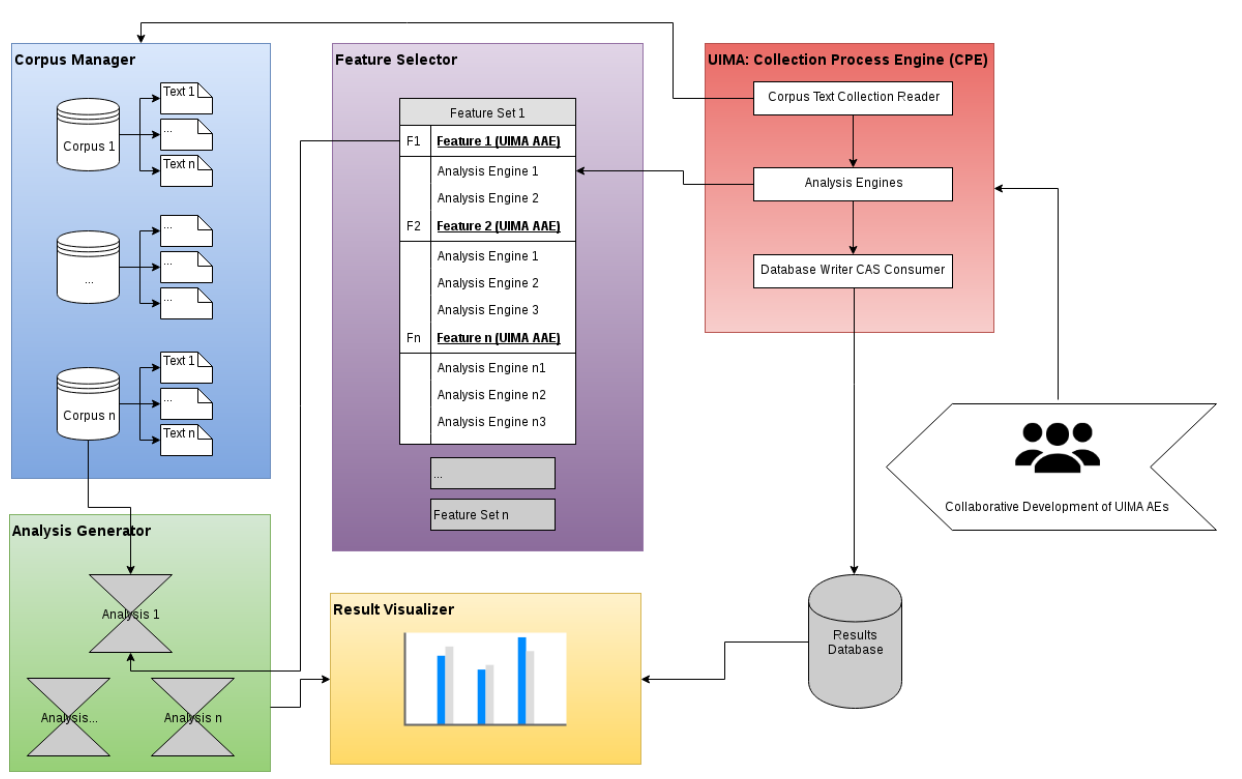
\includegraphics[scale=0.3]{images/ctap.png}
    \caption{Overview of the CTAP architecture. Source: \cite{chen2016-ctap}.}
    \label{fig:ctap}
\end{figure}

CTAP has integrated Portuguese by way of Stanza, the Stanford NLP Group's newly introduced, fully neural, end-to-end NLP pipeline that is compatible with up to 66 languages \citep{qi2020-stanza}. The LingMod Research Group has created a Java wrapper\footnote{\texttt{\url{https://github.com/lingmod-tue/stanza-java}}} around a containerized web service\footnote{\texttt{\url{https://github.com/lingmod-tue/stanza-api}}} hosting Stanza and its model binaries. This effectively lays the groundwork for supporting dozens of other languages out of the box and making CTAP a truly multilingual tool.


\section{Data}
\label{section:data}

The evaluation was conducted on the NLI-PT dataset, a compilation of 3,069 texts by European Portuguese learners originally collected for native language identification \citep{delrio2018, delrio2019a}. Entries are labeled according to their coarse CEFR proficiency level. The raw texts are accompanied by their tokenizations as well as part of speech, constituency, and dependency annotations—none of which were utilized for this analysis in order to make use of CTAP's end-to-end processing pipeline. Entries are labeled according to the corresponding student's native language and CEFR proficiency level group. The detailed breakdown is presented in Table~\ref{tab:nlipt}.

\begin{table}[ht]
\renewcommand{\arraystretch}{1.2}
    \centering
	\resizebox{\columnwidth}{!}{%
    \begin{tabular}{@{}ccccccccccccccccc@{}}
    \toprule
        & {\scshape ara} & {\scshape chi} & {\scshape dut} & {\scshape eng} & {\scshape fre} & {\scshape ger} & {\scshape ita} & {\scshape jap} & {\scshape kor} & {\scshape pol} & {\scshape rom} & {\scshape rus} & {\scshape spa} & {\scshape swe} & {\scshape tet} & {\scshape total} \\
    \midrule
    {\scshape a} & 6 & 133 & 15 & 174 & 42 & 231 & 319 & 34 & 33 & 39 & 45 & 27 & 257 & 16 & 17 & 1,388 \\
    {\scshape b} & 6 & 204 & 20 & 173 & 59 & 149 & 182 & 26 & 9 & 22 & 33 & 59 & 266 & 3 & 4 & 1,215 \\
    {\scshape c} & 2 & 108 & 8 & 68 & 4 & 58 & 64 & 11 & 26 & 16 & 1 & 8 & 91 & 0 & 1 & 466 \\
    \bottomrule
    & 14 & 445 & 43 & 415 & 105 & 438 & 565 & 71 & 68 & 77 & 79 & 94 & 614 & 19 & 22 & 3,069 \\
    \end{tabular}
    }
    \caption{Number of texts in NLI-PT, by CEFR level group and {\scshape l1}.}
    \label{tab:nlipt}
\end{table}

Training, development, and test splits were not defined in the original dataset, and can therefore not be used to directly compare with previous work. Thus, an arbitrary split was generated with \texttt{random\_state=42}. 80\% was used for training with the remaining 20\% for evaluation. The division is further contingent upon CTAP's output, the sequence of which is inconsistent for each run. In addition to the unequal representation of proficiency levels, the texts are based on 148 different tasks also suffering from a heavy class imbalance. Instances are not organized or labeled by their topic.

\section{Methods}

\subsection{Preparation}

CTAP accepts unstructured text as input, so virtually no preprocessing was performed on the corpus. Raw texts were fed into the Corpus Manager and segmented, tokenized, tagged, and dependency parsed with Stanza using models trained on the Universal Dependencies Bosque treebank \citep{rademaker2017-bosque}.

Contractions and otherwise multi-word expressions such as a clitic pronouns as in (\ref{en}, \ref{meso}) needed to be teased apart for part-of-speech tagging and parsing. Expanding surface forms in this way offsets other token boundaries in the original text, wherein the original word's span no longer aligns with those of the newly expanded sentence. The CoNLL-U format is able to represent these multi-word expressions natively during tokenization, which can then be used to update span offsets, greatly simplifying the annotation process. 

In order to preserve surface length features such as the number of characters or number of syllables in the original input text, surface forms need to be stored alongside their underlying tokens. A new surface form analysis engine was therefore added to CTAP to accommodate this discrepancy.

Stanza does not include a constituency parser, which is required for extracting syntactic complexity features. Stanford CoreNLP's Shift-Reduce Parser is a suitable alternative already present in CTAP, but does not offer pre-trained models for Portuguese. LX-Center has released a publicly available model \citep{silva2010}, but it is incompatible with newer versions of the Stanford Parser.

In response, a new model was trained on the CINTIL-Treebank \citep{branco2014-cintil}, after aligning the part of speech tags with the existing UD tagset. Since certain tags were not present in CINTIL, such as {\scshape aux} for auxiliary verbs, these values had to be normalized as well. Phrase and bar-level categories were preserved even when their correlate head projections were modified to fit the UD scheme, as in {\scshape pp} for adpositions ({\scshape adp}) and $\overline{\mbox{{\scshape n}}}$ for nouns ({\scshape noun}).

Customized, language-specific head-finding rules should normally be defined for training a new parsing model. However, a simple left-most head finder has been shown to perform sufficiently well for most tasks \citep{vadas2011-parsing}. For this study, using the \texttt{LeftHeadFinder}\footnote{\texttt{\url{https://nlp.stanford.edu/nlp/javadoc/javanlp/edu/stanford/nlp/trees/LeftHeadFinder.html}}} for training the constituency parser resulted in a surprisingly decent baseline

\subsection{Feature Engineering}

For the complexity analysis, most feature calculations had already been defined for other languages in CTAP and only slight modifications were necessary to include Portuguese. For instance, 21 density features were easily added by declaring the relevant Universal Dependencies tags: Adjective, Adverb, Article, Auxiliary Verb, Cardinal Number, Common Noun, Conjunction, Coordinating Conjunction, Determiner, Function Words, Interjection, Lexical Words, Noun, Particle, Preposition, Punctuation, Pronoun, Proper Noun, Subordinating Conjunction, Symbol, and Verb.

Lexical sophistication measures had also been integrated into CTAP, so it was therefore only necessary to add norm lists for Portuguese. Among them were: age of acquisition \citep{cameirão2010}, concreteness and imageability \citep{soares2016}, familiarity \citep{marques2007}, SUBTLEX frequency information \citep{soares-subtlex}, and discourse markers \citep{mendes2018-ldmpt}. Each of these were calculated on a type or token level, further divided into three categories: lexical words (LW), function words (FW), or both (all words; AW).

Language-agnostic variation features previously discussed in Section~\ref{section:lexical} as well as the remaining lexical features are displayed in Table~\ref{tab:lex}.

\begin{table}
\renewcommand{\arraystretch}{1.2}
    \centering
	\resizebox{\columnwidth}{!}{%
    \begin{tabular}{@{}L{1.25cm}L{6.5cm}L{5cm}@{}}
    \toprule
    \# & {\scshape name} & {\scshape formula} \\
    \midrule
    $f_1$ & TTR & $T/N$ \\
    $f_2$ & RTTR & $T/\sqrt{N}$ \\
    $f_3$ & CTTR & $T/\sqrt{2N}$\\
    $f_4$ & LogTTR & $\log{(T)}/\log{(N)}$\\
    $f_5$ & UberTTR & $\log^{2}{(N)}/\log{(N/T)}$\\
    $f_6$ & MTLD & \cite{mccarthy2010} \\
    \midrule
    \multirow{2}{*}{$f_{7-12}$} & Adjective, Adverb, Lexical Type, Modifier, Noun, Verb & \multirow{2}{*}{$X_{type}/L$} \\
    $f_{13}$ & VV1 & $V_{type}/L$\\
    $f_{14}$ & CVV1 & $V_{type}/\sqrt{2V_{token}}$ \\
    $f_{15}$ & SVV1 & ${V_{type}}^2/V_{token}$\\
    \midrule
    $f_{16-21}$ & Age of Acquisition & \multirow{10}{*}{$X_{type|token}/(N|L|F)$} \\
    $f_{22-27}$ & Concreteness & \\
    $f_{28-33}$ & Familiarity & \\
    $f_{34-39}$ & Imageability & \\
    $f_{40-45}$ & SUBTLEX Word Frequency & \\
    $f_{46-51}$ & SUBTLEX Log Word Frequency & \\
    $f_{52-57}$ & SUBTLEX Contextual Diversity & \\
    $f_{58-63}$ & SUBTLEX Log Contextual Diversity & \\
    $f_{64-69}$ & SUBTLEX Top 1-5k; Below Top 5k & \\
    $f_{70-76}$ & SUBTLEX Zipfian Band 1-7 & \\
    \midrule
    $f_{77-97}$ & POS Density & $X / N$ \\
    \bottomrule
    \end{tabular}
    }
    \caption{Lexical features and their calculations. \textbf{Legend:} $N =$ number of tokens, $T =$ number of types, $L =$ number of lexical tokens, $F =$ number of function tokens.}
    \label{tab:lex}
\end{table}

There are 21 dependency-based features, 14 general constituency counts, and 42 syntactic complexity ratios available for Portuguese. The rules for extracting constituency phenomena were defined using Tregex \citep{tregex}.

Some morphosyntactic features have been added specifically for Portuguese. Clitic usage \citep{flores2014, costa2015}, mood \citep{flores2016, jesus2019}, and clefts \citep{lobo2019} are systems that have been demonstrated to follow certain development patterns and may correlate with {\scshape l2} proficiency growth.

Table~\ref{tab:msy} catalogues all morphosyntactic features, with Portuguese clefts appearing separately in Table~\ref{tab:tregex} to demonstrate a subset of Tregex rules.

\begin{table}[h]
\renewcommand{\arraystretch}{1.2}
    \centering
	\resizebox{\columnwidth}{!}{%
    \begin{tabular}{@{}L{1.25cm}L{9cm}L{2.5cm}@{}}
    \toprule
    \# & {\scshape name} & {\scshape formula} \\
    \midrule
    $f_{98-118}$ & Dependency Locality Theory & \cite{gibson2000} \\
    $f_{119-139}$ & Number of phrasal, clausal, or sentential constituents & $X$\\
    $f_{140-137}$ & Mean length of phrase, clause, or T-Unit & $W/X$ \\
    $f_{138-142}$ & Clausal, sentential, and T-Unit complexity ratios & Variable \\
    \midrule
    \multirow{3}{*}{$f_{143-151}$} & Complex Nominal, Complex T-Unit, Coordinate Phrase, Dependent Clause, NP, PP, Relative Clause, Verb Cluster, VP & \multirow{3}{*}{$X/S$}\\
    \multirow{2}{*}{$f_{152-158}$} & Complex Nominals, Coordinate Phrase, NP, PP, Relative Clause, Verb Cluster, VP & \multirow{2}{*}{$X/CL$}\\
    \multirow{2}{*}{$f_{159-166}$} & Complex Nominal, Coordindate Phrase, Dependent Clause, NP, PP, Relative Clause, Verb Cluster, VP & \multirow{2}{*}{$X/TU$} \\
    $f_{167-168}$ & Prenominal Modifer, Postnominal Modifier & $X/NP$\\
    \midrule
    \multirow{2}{*}{$f_{169-174}$} & Conditional, Imperfect, Inflected Infinitive, Pluperfect, Preterite, Subjunctive & \multirow{4}{*}{$X/VP$} \\
    $f_{175-178}$ & Proclitic, Enclitic, Mesoclitic, All & \\
    $f_{179-183}$ & Clefts & \\
    \bottomrule
    \end{tabular}
    }
    \caption{Morphosyntactic features. \textbf{Legend:} $W =$ number of words, $S= $ number of sentences, $CL =$ number of clauses, $TU =$ number of T-Units.}
    \label{tab:msy}
\end{table}

\begin{table}
\renewcommand{\arraystretch}{1.2}
    \centering
	\resizebox{\columnwidth}{!}{%
    \begin{tabular}{@{}L{1.25cm}L{4cm}L{7.5cm}@{}}
    \toprule
    \# & {\scshape name} & {\scshape tregex pattern} \\
    \midrule
    \multirow{4}{*}{$f_{184}$} & \multirow{4}{*}{\textit{é que} Clefts} & \texttt{S|VP [< ((VP|VERB|AUX [{<<} /[Éé]/]) [\$+ ((CP [< ((SCONJ [< /[Qq]ue/]))]) [< (SCONJ [\$+ S])])])]}\\
    \midrule
    \multirow{4}{*}{$f_{185}$} & \multirow{4}{*}{It-Clefts} & \texttt{S|VP [< ((VP|VERB|AUX [{<<} COPULA]) [\$+ ((NP [!< (PRON [< /[Oo]/])]) [< (N' [< (CP|NP [< ((NP < PRON) [\$+ S|NP])])])])])]}\\
    \midrule
    \multirow{4}{*}{$f_{186}$} & \multirow{4}{*}{Pseudoclefts} & \texttt{S|VP [ < ((NP [< ((NP < (PRON [< /[Oo]|[Qq]uem/])) [\$+ S|NP])]) [\$+ (S|VP [{<<} (VP|VERB|AUX [<1 COPULA])])])]}\\
    \midrule
    \multirow{3}{*}{$f_{187}$} & \multirow{3}{*}{Inverted Pseudoclefts} & \texttt{S|VP [< ((VP|VERB|AUX [{<<} COPULA]) [\$+ (NP [<<, (PRON < /[Oo]|[Qq]uem/)] [< N'|CP|S])])]} \\
    \midrule
    \multirow{4}{*}{$f_{188}$} & \multirow{4}{*}{WH-Clefts} & \texttt{(S|VP [< ((VP|VERB|AUX [{<<} COPULA]) [\$+ NP])]) [\$+ (NP [< ((NP < PRON) [\$+ (S [< (NP [\$+ VP])])])])]} \\
    \bottomrule
    \end{tabular}
    }
    \caption{Tregex rules for syntactic complexity based on a constituency parse generated with UD-Bosque tags and left head-finding rules. COPULA refers to the regular expression pattern matching any relevant copular form: \texttt{/[Éé]|
    [Ff](o(i|r(am?|em)?|ssem?))|[Ee]ram?|[Ss](e(r(iam?|ão|á)|jam?)| ão|ido)/}}
    \label{tab:tregex}
\end{table}

\pagebreak

Cohesion measures are incorporated through both the raw tallies of different classes of connectives (see Section~\ref{section:coh}) as well as ratios indicating the usage of certain types in relation to the total number of connectives. Also taken into account are the proportion of single-word and multi-word phrasal connectives.

\begin{table}[H]
\renewcommand{\arraystretch}{1.2}
    \centering
	\resizebox{\columnwidth}{!}{%
    \begin{tabular}{@{}L{2cm}L{5.5cm}L{5.5cm}@{}}
    \toprule
    \# & {\scshape name} & {\scshape formula} \\
    \midrule
    $f_{189-196}$ & Number of connectives & $X$ \\
    $f_{197-206}$ & Cohesive complexity & $X/(N|CO)$ \\
    \bottomrule
    \end{tabular}
    }
    \caption{Cohesion measures. \textbf{Legend:} $N =$ number of tokens, $CO =$ number of connectives.}
    \label{tab:coh}
\end{table}

The remaining 20 measures are global, require little to no linguistic insight, and are calculated straightforwardly. Finally, 15 native languages are represented in the corpus. These were included as categorical features, summing to a total of 241 features.

\begin{table}[b!]
\renewcommand{\arraystretch}{1.2}
    \centering
	\resizebox{\columnwidth}{!}{%
    \begin{tabular}{@{}L{2cm}L{11cm}@{}}
    \toprule
    \# & {\scshape name} \\
    \midrule
    $f_{207-208}$ & Standard deviation: token length (syllable, letter) \\
    $f_{209-211}$ & Standard deviation: sentence length (syllable, letter, token) \\
    $f_{212-213}$ & Number of word type, token with 2+ syllable \\
    $f_{214-215}$ & Percent word type, token with 2+ syllable \\
    \multirow{2}{*}{$f_{216-221}$} & Number of letters, syllables, surface forms, tokens, token types, sentences \\
    $f_{222-223}$ & Mean token length: syllable, letter \\
    $f_{224-226}$ & Mean sentence length: syllable, letter, token \\
    \midrule
    $f_{226-241}$ & Native language (categorical) \\
    \bottomrule
    \end{tabular}
    }
    \caption{Shallow complexity features and {\scshape l1}.}
    \label{tab:shallow}
\end{table}

%%%%%%%%%%%%%%%%%%%%%%%%%%%%%%%%%%%%%%
%%%%%%%%%%%%%%%%%%%%%%%%%%%%%%%%%%%%%%
%%%%%%%%%%%%%%%%%%%%%%%%%%%%%%%%%%%%%%

\subsection{Supervised Machine Learning}

Traditional machine learning methods have been commonly used for several CEFR level classification tasks, and have generally performed quite well \citep{vajjala2014-estonian, pilan2016-swedish, vajjala2017-features, delrio2019a}. Experiments for this linguistic complexity analysis of {\scshape l2} Portuguese were performed with Random Forests, Support Vector Machines, and Logistic Regression using the scikit-learn library \citep{scikit-learn}.

For each system, hyperparameters were tuned using grid search and 10-fold cross-validation. Feature calculations were scaled to mitigate the effect of high cardinality values, which introduce bias against features with lower value ranges during training. Finally, ablation tests were performed by assessing the systems on different feature subsets to observe the performance of each combination.

\subsection{Feature Selection}

There are multiple calculations that measure similar if not the same metric. For example, the number of surface forms and the number of tokens are very highly correlated. Though usually not a bijective relation, these two features increase almost collinearly. This sort of redundancy should be avoided. Instead, distinct and complementary features have been argued to capture a more diverse, holistic picture of one's {\scshape l2} system \citep{norris2009}. Care was therefore taken to prune undesirable features and reduce model variance prior to evaluation.

Correlation-based feature subset selection \citep[CfsSubsetEval;][]{hall1998} from the WEKA library \citep{weka} was employed to incrementally purge highly correlated features, while retaining those with higher predictive ability of the class. Out of the 241 available features, including each student's native language, 53 were returned, all of which are catalogued in Table~\ref{tab:subsetfeatures}. Relevant features will be elaborated on in Section~\ref{section:discussion}.

\begin{table}%[H]
\renewcommand{\arraystretch}{1.2}
    \centering
    \resizebox*{!}{0.95\textheight}{%
    \begin{tabular}{@{}L{1.25cm}L{1cm}l@{}}
        \toprule
         $f_{1-2}$ & {\scshape sur} & Mean Sentence Length in Letters, Tokens \\
         $f_3$ & {\scshape sur} & Mean Token Length in Syllables \\
         $f_4$ & {\scshape sur} & Number of Letters \\
         $f_5$ & {\scshape sur} & Percentage of Tokens with More Than 2 Syllables \\
         $f_6$ & {\scshape sur} & Percentage of Word Types with More Than 2 Syllables \\
         $f_7$ & {\scshape sur} & SD Sentence Length in Letters \\
         $f_8$ & {\scshape sur} & SD Token Length in Letters \\
        \midrule
         $f_{9-11}$ & {\scshape lex} & Age of Acquisition (AW Token; AW, LW Type) \\
         $f_{12-14}$ & {\scshape lex} & Concreteness (AW, FW Token; LW Type) \\
         $f_{15-17}$ & {\scshape lex} & Familiarity (AW, LW Type; LW Token) \\
         $f_{18-20}$ & {\scshape lex} & Imageability (AW Token; AW, LW Type) \\
         $f_{21}$ & {\scshape lex} & SUBTLEX Contextual Diversity (FW Token) \\
         $f_{22-25}$ & {\scshape lex} & SUBTLEX Frequency Band 2, 3, 4, 5 \\
         $f_{26}$ & {\scshape lex} & SUBTLEX Frequency Below Top 5000 \\
         $f_{27-29}$ & {\scshape lex} & SUBTLEX Log Word Frequency (AW Token; AW, FW Type) \\
         $f_{30-32}$ & {\scshape lex} & SUBTLEX Word Frequency (AW, FW Type; FW Token) \\
         $f_{33}$ & {\scshape lex} & Corrected Verb Variation 1 \\
         \multirow{2}{*}{$f_{34-38}$} & \multirow{2}{*}{{\scshape lex}} & POS Density: Cardinal Number, Interjection, \\
         & & Punctuation, Subordinating Conjunction, Symbol \\
        \midrule
         $f_{39}$ & {\scshape msy} & ``é que" Cleft per VP \\
         $f_{40}$ & {\scshape msy} & Dependent Clause per Clause \\
         $f_{41} $ & {\scshape msy} & Dependent Clause per Sentence \\
         $f_{42}$ & {\scshape msy} & Clause per T-unit \\
         $f_{43}$ & {\scshape msy} & Mean Length of Noun Phrase \\
         \multirow{2}{*}{$f_{44-46}$} & \multirow{2}{*}{{\scshape msy}} & Number of Dependent Clauses, It-Clefts, \\
         & &  Prenominal Noun Modifiers \\
         $f_{47}$ & {\scshape msy} & Number of Proclitics per VP \\
         $f_{48-49}$ & {\scshape msy} & Verb per VP: Inflected Infinitive, Subjunctive \\
        \midrule
         $f_{50-51}$ & {\scshape coh} & Connectives per Token: Additive, Concessive \\
         $f_{52} $ & {\scshape coh} & Number of Connectives \\
        \midrule
         $f_{53} $ & {\scshape l1} & Russian \\
        \bottomrule
    \end{tabular}
    }
    \caption{All features returned by CfsSubsetEval, unranked.}
    \label{tab:subsetfeatures}
\end{table}

Table~\ref{tab:infogain} ranks the best features by their information gain. Many of the features appearing in this list have been connected to a more complex language system. The number of letters (\#1) is a general length-based measure that has been shown to be a powerful indicator when paired with other finer-grained measures \citep{norris2009}. \Citet{ortega2012} asserts that complex noun phrases such as (\#3) are characteristic of advanced learners, and had previously found that the amount of subordination as in (\#6) is relevant \citep{wq1998, ortega2003}. Finally, \cite{lu2012} concluded that CVV1 (\#9) is among the best features for assessing lexical variation.

\begin{table}[b!]
\renewcommand{\arraystretch}{1.2}
    \centering
    \begin{tabular}{@{}L{1cm}l@{}}
        \toprule
        {\scshape \#} & {\scshape feature name} \\
        \midrule
        1 & Number of Letters \\
        2 & Imageability (AW Type) \\
        3 & Number of Prenomial Noun Modifier \\
        4 & Imageability (LW Type) \\
        5 & SUBTLEX Word Frequency (AW Type) \\
        6 & Number of Dependent Clauses \\
        7 & Concreteness (LW Type) \\
        8 & Age of Acquisition (LW Type) \\
        9 & Corrected Verb Variation 1\\
        10 & Concreteness (AW Token) \\
        \bottomrule
    \end{tabular}
    \caption{Top 10 features ranked by information gain according to CfsSubsetEval.}
    \label{tab:infogain}
\end{table}

The remaining features are based on lexical sophistication. A plethora of these measures are also present in the entire returned feature subset. These broadly measure the use of ``advanced" words—often corresponding to lower frequency—that demonstrate higher lexical proficiency \citep{crossley2017}. More than half of the top ten features by information gain are related to lexical sophistication: imageability (all and lexical word types), word frequencies (all word types), concreteness (all and lexical word types), and age of acquisition (lexical  word types). \Citet{crossley2012} found that imageability was the strongest predictor of all which is in line with the results returned by CfsSubsetEval, being the second best feature after the general length measure. \Citet{chen2017} also assert that averaging word frequency information using frequency bands characterizes text readability, especially when normalized. Four different Zipfian bands appear, excluding the first band of highly frequent words as well as the lowest bands containing the most rare and obscure ones. Several other frequency features from the SUBTLEX corpus are relevant, further stressing the importance of lexical frequency in measuring growth.

There are many other language-agnostic features returned by CfsSubsetEval that have been established as anchors for complexity analyses in other languages. Notable are the Corrected Verb Variation 1 \citep{lu2012, vajjala2014-estonian}, density of interjections and subordinating conjunctions \citep{vajjala2014-estonian}, dependent clauses per clause \citep{bulte2012}, and clause per T-unit \citep{vyatkina2012}.


\section{Results}

Average scores for 10-fold cross validation are reported along with the held-out test set. Following \cite{delrio2019a}, accuracy is used as the main evaluation metric with F1-score also provided due to the class imbalance. Since there is no test set provided by NLI-PT, direct comparisons are not possible.

For individual feature groups, lexical features are the clear winner. This is also the largest class with 97 different calculations. Morphosyntactic features perform only slightly better than surface ones, even with a 51-feature disparity between the two, showing that surface features alone can explain a large amount of variance between proficiency levels. Cohesive devices are also able to exceed naïve baselines and score similarly to surface features, but are generally the weakest set.

Using the feature subset provided by CfsSubsetEval, accuracy scores are on par with the entire feature set, though the F1-score reveals a noticeable dip when accounting for the class imbalance. Logistic Regression and SVMs are best when using all features, but Random Forests score better when using the subset.

\pagebreak

\vspace{\fill}

\begin{table}[H]
\renewcommand{\arraystretch}{1.2}
    \centering
    \begin{tabular}{@{}lC{1cm}C{1cm}cccc}
    \toprule
        & \multirow{2}{*}{{\scshape kind}} & \multirow{2}{*}{{\scshape size}} & \multicolumn{2}{c}{{\scshape 10-fold cv}} & \multicolumn{2}{c}{{\scshape test}} \\
        & & & {\scshape $\mu$-f1} & {\scshape $\mu$-acc} & {\scshape f1} & {\scshape acc} \\
        \midrule
        Random Baseline & & & 0.33 & 0.33 & 0.33 & 0.33 \\
        Majority Baseline & & & 0.20 & 0.45 & 0.20 & 0.45 \\
        \midrule
        Random Forest & \multirow{3}{*}{{\scshape sur}} & \multirow{3}{*}{20} & 0.50 & 0.62 & 0.49 & 0.61 \\
        Logistic Regression & & & 0.46 & 0.63 & 0.47 & 0.63 \\
        Support Vector Machine & & & 0.46 & 0.63 & 0.44 & 0.62 \\
        \midrule
        Random Forest & \multirow{3}{*}{{\scshape lex}} & \multirow{3}{*}{97} & 0.56 & 0.67 & 0.55 & 0.65 \\
        Logistic Regression & & & \textbf{0.57} & \textbf{0.66} & \textbf{0.57} & \textbf{0.68} \\
        Support Vector Machine & & & \textbf{0.57} & \textbf{0.66} & \textbf{0.57} & 0.64 \\
        \midrule
        Random Forest & \multirow{3}{*}{{\scshape msy}} & \multirow{3}{*}{71} & 0.50 & 0.63 & 0.53 & 0.65 \\
        Logistic Regression & & & 0.48 & 0.63 & 0.47 & 0.62 \\
        Support Vector Machine & & & 0.47 & 0.64 & 0.48 & 0.64 \\
        \midrule
        Random Forest & \multirow{3}{*}{{\scshape coh}} & \multirow{3}{*}{18} & 0.45 & 0.56 & 0.50 & 0.59 \\
        Logistic Regression & & & 0.44 & 0.61 & 0.44 & 0.61 \\
        Support Vector Machine & & & 0.44 & 0.61 & 0.44 & 0.62 \\
    \bottomrule
    \end{tabular}
    \caption{Trials using surface, lexical, morphosyntactic, and cohesive feature sets.}
    \label{tab:results}
\end{table}

\vspace{\fill}

\pagebreak

\begin{table}[H]
\renewcommand{\arraystretch}{1.2}
    \centering
    \begin{tabular}{@{}lC{1cm}C{1cm}cccc}
    \toprule
        & \multirow{2}{*}{{\scshape kind}} & \multirow{2}{*}{{\scshape size}} & \multicolumn{2}{c}{{\scshape 10-fold cv}} & \multicolumn{2}{c}{{\scshape test}} \\
        & & & {\scshape $\mu$-f1} & {\scshape $\mu$-acc} & {\scshape f1} & {\scshape acc} \\
        \midrule
        Random Baseline & & & 0.33 & 0.33 & 0.33 & 0.33 \\
        Majority Baseline & & & 0.20 & 0.45 & 0.20 & 0.45 \\
        \midrule
        Random Forest & \multirow{3}{*}{{\scshape cse}} & \multirow{3}{*}{53} & 0.56 & 0.67 & 0.58 & 0.68 \\
        Logistic Regression & & & 0.58 & 0.67 & 0.56 & 0.68 \\
        Support Vector Machine & & & 0.59 & \textbf{0.68} & 0.55 & 0.66 \\
        \midrule
        Random Forest & \multirow{3}{*}{{\scshape all}} & \multirow{3}{*}{241} & 0.56 & 0.67 & 0.54 & 0.67 \\
        Logistic Regression & & & 0.59 & 0.67 & \textbf{0.61} & \textbf{0.69} \\
        Support Vector Machine & & & \textbf{0.62} & \textbf{0.68} & \textbf{0.61} & 0.67 \\
    \bottomrule
    \end{tabular}
    \caption{Scores achieved by systems using CfsSubsetEval (CSE) vs. all features.}
    \label{tab:results}
\end{table}

\vspace{\fill}

The confusion matrix for the test set in Table~\ref{tab:cm} shows that CEFR-A is the easiest class to predict, with CEFR-B faring slightly worse. CEFR-C is by far the worst predicted class, with an outright majority of instances being classified as its lower neighbor, followed by CEFR-A.

\vspace{\fill}

\begin{table}[H]
\renewcommand{\arraystretch}{1.2}
    \centering
    \begin{tabular}{@{}lrrr@{}}
    \toprule
        Pred &    {\scshape a} & {\scshape b} & {\scshape c} \\
        True &      &      &     \\
        \midrule
        {\scshape a} &  \textbf{225} &   48 &   5 \\
        {\scshape b} &   58 &  \textbf{177} &   8 \\
        {\scshape c} &   26 &  \textbf{53}  &  14 \\
    \bottomrule
    \end{tabular}
    \caption{Confusion matrix for Logistic Regression.}
    \label{tab:cm}
\end{table}

\vspace{\fill}
\section{Discussion}
\label{section:discussion}

\subsection{Portuguese Features}

The Portuguese clitic system is complex, with various phonological and syntactic constraints governing their form and position. Usually, object pronouns are realized as enclitics, immediately succeeding a verb attached by a hyphen as in (\ref{enc}). Proclitics, however, are required in situations affected by subordination, interrogation, quantification, negation, and aspect \citep{flores2014}. In this case, the object pronoun precedes the verb, and is not attached by a hyphen as in (\ref{neg}).

\begin{exe}
\ex\label{enc}
\gll Ele viu-o \\
he see.{\scshape 3.sg.past}={\scshape 3.sg.masc}\\
\glt ``He saw him" \citep{flores2014}

\ex\label{neg}
\gll O João não {a viu} \\
the João not {\scshape 3.sg.fem}=see.{\scshape 3.sg.past} \\
\glt ``João never saw her" \citep{flores2014}
\end{exe}

Due to these restrictions, it has been found that early learners generalize enclisis, and later acquire the contexts which call for proclisis \citep{flores2014}. The reverse has not been observed, however: proclisis is never generalized in situations of enclisis.\footnote{It is worth noting that this is characteristic of European Portuguese in particular, on which the learner corporus is based, as the converse is true for Brazilian Portuguese: proclisis is generally preferred in most contexts with enclisis being considered formal, pedantic, or even archaic \citep{galves2005, simoes2006}. This also explains the acceptability of (\ref{pro}) in Section~\ref{section:pt}; strictly speaking, proclisis is canonically forbidden in the sentence-initial position, with Brazilian Portuguese having adopted looser conditions on such placement.}

The results of the feature analysis for these two patterns are revealed in Figure~\ref{fig:clitics}. Enclitic distribution is similar across proficiency levels, whereas proclitics are clearly picked up later. Even with many outliers, proclisis in CEFR-A is very close to zero on average. The rate increases gradually in CEFR-B and even moreso in CEFR-C, with fewer outliers appearing in each class.

\begin{figure}
\centering
\begin{subfigure}{1.0\textwidth}
  \centering
  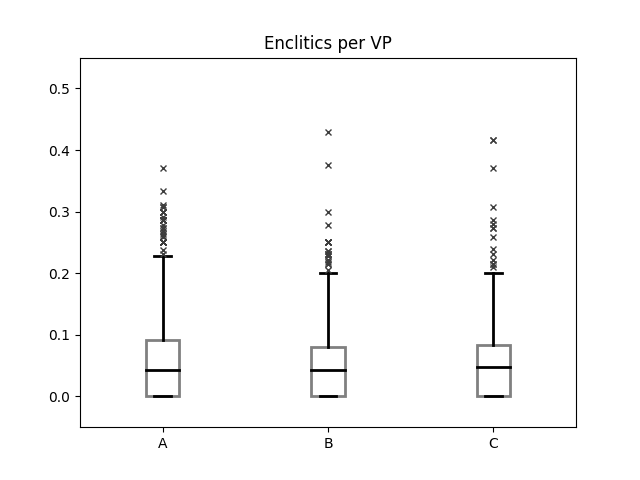
\includegraphics[width=0.9\linewidth]{images/enc.png}
\end{subfigure}%

\begin{subfigure}{1.0\textwidth}
  \centering
  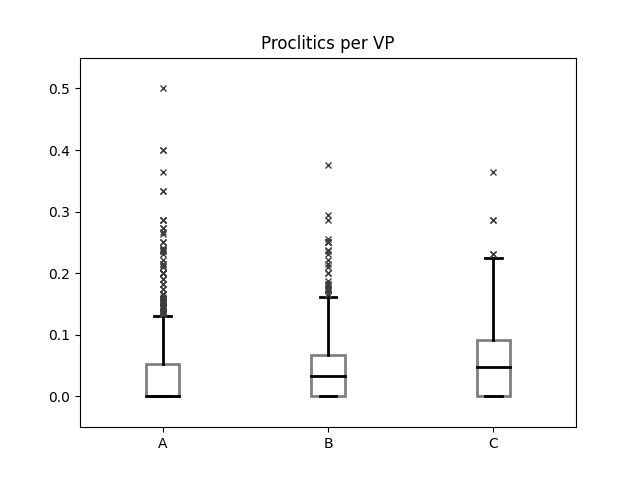
\includegraphics[width=0.9\textwidth]{images/proc.png}
\end{subfigure}
\caption{Use of clitic constructs in NLI-PT.}
\label{fig:clitics}
\end{figure}

It follows that the number of proclitics employed is better correlated with proficiency level than enclitic use, as indicated by CfsSubsetEval. This corroborates the claim that proclitics are acquired in a later stage of development \citep{flores2014, costa2015}.

Curiously, the elusive mesoclitic is absent from the feature list. Being restricted to the future and conditional tenses, there are fewer opportunities for its use. The arcane manner in which it must split a verbal stem from its inflection may also deter students, preferring instead the more familiar clitic varieties. Indeed, average use rates for mesoclitics are near-zero for all levels, with only a handful of outliers almost equally distributed across classes, negating any potential effect.

Moving on to verbal morphology, two inflectional paradigms of interest make an appearance in CfsSubsetEval: the subjunctive mood, a pattern difficult for many students learning Romance languages, and the extremely rare inflected infinitive, present in few other languages.

The inflected infinitive is an unusual form that allows for person and number agreement with an untensed verb. There is always a grammatically-licensed finite alternative, meaning their use is never mandatory \citep{iverson2008}. \Citet{rothman2010, rothman2013} have suggested that these patterns are acquired by late childhood, but may still cause problems even for adults who may accept certain pragmatic cues and draw inferences that alter the intended meaning of the utterance. Unfortunately, most research on this phenomenon have focused on monolingual native speakers in {\scshape l1} acquisition.

The usage distribution across proficiency levels in NLI-PT is seemingly random, with no general trend in increased usage for higher proficiency levels. It is possible that, since the first and third person singular forms are inflected with a null morpheme and are therefore homographs with each other as well as their uninflected form, this could be either unintended use by the student or even misidentified by the Stanza parser. These conjectures, however, still do not explain its predictive value according to CfsSubsetEval, other than the fact that it is not strongly correlated to other input variables.

Subjunctive, on the other hand, is much easier to interpret. Romance languages are well known for their extensive verbal morphology which can be overwhelming for students coming from an {\scshape l1} without such variation. Furthermore, this mood is employed in non-epistemic situations that would otherwise make use of the indicative. While commonly triggered by certain verbs such as \textit{querer} ``to want", it may be difficult to identify when required by less common or more opaque predicates \citep{flores2016, jesus2019}.

Beginner students are less likely to use the subjunctive, being introduced to it at an intermediate stage. This is clearly evident in the distribution in NLI-PI, illustrated in Figure~\ref{fig:subjunctive}. The vast majority of level A students do not use subjunctive at all, even though there are many outliers. However, the distribution between levels B and C are almost the same, though slightly less for the more advanced. This could be due to the fact that this mood is introduced and practiced more at the intermediate stage. The distribution indicates that it is a good proxy by which to discriminate between beginner texts and the higher levels.

\begin{figure}[H]
    \centering
    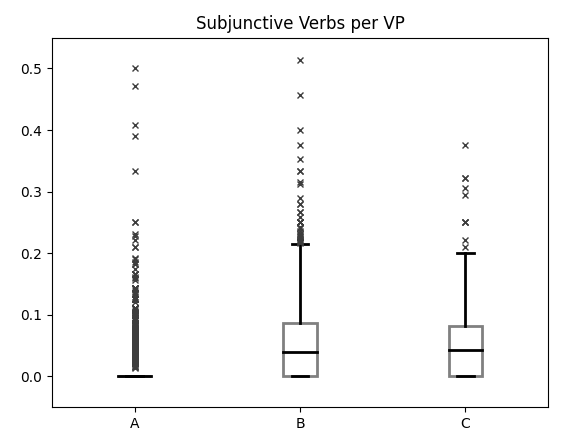
\includegraphics[width=0.8\textwidth]{images/svp.png}
    \caption{Use of subjunctive in NLI-PT.}
    \label{fig:subjunctive}
\end{figure}

The various clefting strategies available in Portuguese give rise to the potential for great syntactic variation. Of the five cleft constructions described in Section~\ref{section:pt}, only two were identified often enough in the corpus to make any impact: it-clefts and \textit{é que} clefts. \textit{WH}-clefts were not found at all, and the remaining pseudoclefts and inverted pseudoclefts were sparse. However, this may be the result of poor tagging and parsing of the learner texts using models trained on native text, and consequently the possibly unintuitive matching patterns described in Table~\ref{tab:tregex}, which were designed for the parsing model trained using simple left head-finding rules.

\Citet{lobo2015} found that both it-clefts and \textit{é que} clefts are acquired earlier than the remaining varieties and are generally widespread in child speech. In NLI-PT, standard clefts are used less frequently overall than \textit{é que} clefts, but the former is employed similarly across proficiency levels compared to the latter, which appears more often in higher proficiency levels. This also suggests that it is helpful in classifying higher levels compared to CEFR-A.

Interestingly, few features appear that target morphology, which would have been expected given the highly inflectional nature of Portuguese in addition to the results obtained by \cite{vajjala2014-estonian} for Estonian, which conclude that morphological features can be highly predictive. \Citet{delrio2019a}'s use of POS \textit{n}-grams with fine-grained morphological information seems to fill this gap, with \cite{vajjala2018-cefr} also observing promising results using word and POS \textit{n}-grams, though \cite{vajjala2014-estonian} reported low scores using POS \textit{n}-grams.

Encoding native language as a categorical feature has also been postulated to be a useful feature in proficiency classification \citep{vajjala2017-features}, but no information gain was observed in this study with the exception of Russian being the only one to appear as a viable {\scshape l1} feature. This is an interesting development, since certain vocabulary and syntactic choices may be characteristic of a particular {\scshape l1} and may have potential transfer effects. For example, Spanish speakers may be expected to produce a higher rate of grammatical sentences even at lower levels given the close proximity between the two languages. This substantiates \cite{crossley2011}, having shown homogeneity between learners of varying {\scshape l1}s.

\subsection{Comparisons}

\Citet{delrio2019a} in her first experiments with Portuguese proficiency classification found complexity measures, which she refers to as ``descriptive" features, among the weakest predictors, with the best scores being achieved using bag-of-words and POS \textit{n}-grams. However, the set of approximately 39 complexity features she used is much smaller than the amount employed in this study.

Later, \cite{delrio2019b} obtained generally poor results in her experiments training systems on Spanish for cross-lingual classification, though there are a few interesting takeaways. While bag-of-words, POS, and dependency linguistic features outperform complexity features, their interclass results are quite inconsistent with lows ranging from 0.19 F-1 macro for classifying CEFR-B with dependency n-grams, to 0.68 F-1 macro in CEFR-A using POS n-grams. CEFR-C was not able to be classified with these features at all, scoring 0.0 F1-macro across the board. Complexity features, however, are more stable: general measures scored a high of 0.60 F1-macro for A, with other subsets scoring between 0.40 and 0.48. Among levels B and C, F1 scores are almost the same for all subsets: 0.48-0.49 for B and 0.25-0.30 for C. This suggests that, while the small set of complexity features on their own may not have been the best, they are still insightful as predictive variables.

Combining these complexity measures with POS \textit{n}-grams resulted in further accuracy gains for classes A and B, though F1 scores for level C surprisingly plummeted back to 0.0. Given that the best results she observed for Spanish monolingual classification, however, were achieved through a combination of POS \textit{n}-grams and a larger amount of complexity features, it follows that using these in tandem for monolingual Portuguese classification could lead to improved scores.

\subsection{Detractors}
\label{section:detractors}

Recall that linguistic complexity and accuracy are separate entities in the CAF triad for measuring second language acquisition \citep{housen2009}. While complexity focuses on elaborateness and variation in learner expression, it is not concerned with errors made by students. However, the veracity of these feature calculations is susceptible to grammar and mechanical errors. Incorrect orthography or word choice obfuscates the student's intent, leading to incorrect tagging and parses and a contaminated analysis.

For example, one CEFR-A student achieved an impressive 50\% subjunctive verb usage per verb phrase, clearly visible in Figure~\ref{fig:subjunctive}. The subjunctive mood is often acquired later and it is therefore unlikely that a student would be capable of producing this construct so early, much less as often as was indicated. Upon closer inspection, it appears that this student—whose native language is Spanish—erroneously used the subjunctive present forms \textit{tome} and \textit{volte} instead of the indicative past \textit{tomei} and \textit{voltei}, which is clearly negative transfer from Spanish simple past, e.g. \textit{tomé}.

In the previous example, the verbal inflection was correctly identified, tagged, and parsed even though it was used incorrectly. Other situations result in a bad parse that propagates throughout the pipeline, culminating with an incorrect parse tree and, accordingly, inaccurate feature calculations. Sentence (\ref{sconj}) illustrates one such instance. The verb \textit{tendem} takes the optional prepositions \textit{a} or \textit{para} depending on context. This student has introduced an inappropriate preposition \textit{de} that is labeled by a confused tagger as a subordinate conjunction in what is really a simple sentence with no subordination.

\begin{exe}
\ex[*] {\label{sconj}
Os actores tendem de ser mais dramáticos também \\
The actors tend to to be more dramatic too}
\end{exe}

While Stanza otherwise provides a fairly competent parse of input text and relatively high accuracy is generally achieved for tokenization, tagging, lemmatization, and dependency parsing, there are still some shortcomings due to its data-driven approach and comparably smaller training set. For example, it seems that mesoclitics are not well-represented in the UD training corpus, because they are often poorly tokenized. This can be minor, as is the case with \textit{telefonar-lhes-ia} ``I would call them", which is split into \textit{telefonará} + \textit{lhes}, changing the tense from conditional to future. In other situations, it can result in very obscure results, such as merging an object pronoun with the inflected verb, introducing a new pronoun that was not present in the original mesoclitic, or even creating a brand new word not licensed by the language. This was resolved by creating hard-coded rules, searching for up to two object pronouns between hyphens and an inflectional suffix from one of the two appropriate tenses.

Another example would be the adverbial modifier ``how" and the first person singular conjugation of ``to eat", which are homonymous: \textit{como}. Only the former is represented in the UD training set which naturally leads to a questionable tag in a situation where the verb is clearly required. The parse tree for a sentence affected by this is depicted in Figure~\ref{fig:tree}.

\begin{figure}%[H]
\centering
    \tikzset{frontier/.style={distance from root=90pt}}
    \resizebox{\columnwidth}{!}{%
    \Tree[. \node{{\scshape s}}; 
        [. \node{{\scshape adv}}; 
        [. \node{\textit{Normalmente}}; ] ] 
        [. \node{{\scshape s}}; 
        [. \node{{\scshape np}}; 
        [. \node{{\scshape pron}}; 
        [. \node{\textit{eu}}; ] ] ]
        [. \node{{\scshape *s{\ \ }}}; 
        [. \node{{\scshape *pp{\ \ }}}; 
        [. \node{{\scshape *adp{\ \ }}}; 
        [. \node{\textit{como}}; ] ]
        [. \node{{\scshape np}}; 
        [. \node{{\scshape noun}};
        [. \node{\textit{torrada}}; ] ] ] ] 
        [. \node{{\scshape *s{\ \ }}}; 
        [. \node{{\scshape cconj}}; 
        [. \node {\textit{e}}; ] ]
        [. \node{{\scshape s}}; 
        [. \node{{\scshape vp}}; 
        [. \node{{\scshape verb}}; 
        [. \node{\textit{bebo}}; ] ] 
        [. \node{{\scshape np}};
        [. \node{$\overline{\mbox{{\scshape n}}}$};
        [. \node{{\scshape noun}}; 
        [. \node{\textit{café}}; ] ]
        [. \node{{\scshape pp}}; 
        [. \node{{\scshape adp}}; 
        [. \node{\textit{com}}; ] ] 
        [. \node{{\scshape np}}; 
        [. \node{{\scshape noun}};
        [. \node{\textit{leite}}; ] ] ] ] ] ] ] ] ] ] ] ]
        }
    \caption{Constituency tree for ``Normally I eat toast and drink coffee with milk". The verb \textit{como} ``eat" is mistaken for its prepositional homonym, projecting to a prepositional phrase instead of a verbal phrase. The error percolates to the sentence conjunct, which should be a complementizer phrase.}
    % Original text: \texttt{eng\_A\_031CVITF\_2\_cop.txt}.
    \label{fig:tree}
\end{figure}

Incorporating learner errors could provide a further dimension in which to better predict proficiency level. \Citet{vajjala2017-features, weiss2019-german} both found that errors in conjunction with complexity features were useful in their proficiency classification experiments. Further, \citet{delrio2019a} hypothesized that bag-of-words performed strongest for Portuguese proficiency classification because it can help identify orthographic mistakes. POS \textit{n}-grams, which were the next best feature in isolation, are also able to capture, for example, agreement errors in gendered nouns and adjectives. Both of these performed better in her experiments over the linguistic complexity features, so combining their effects with the augmented complexity feature set introduced in this work could be beneficial, as would incorporating other error patterns such as the incorrect expansion of mandatory contractions (see Section~\ref{section:pt}) and allomorphic variation of clitics.

Task variation may also negatively impact the classifier due to varied learner language across different prompts. As mentioned in Section~\ref{section:data}, texts are not labeled according to their associated topic and resolving topics from the texts themselves is non-trivial. Since linguistic complexity analyses are sensitive to the topic around which each text is based, as varied writing prompts can elicit different language patterns \citep{ventura2015, yang2015}, this has the potential to adversely influence the analysis because similar tasks cannot be grouped together during evaluation.

\subsection{Proficiency Levels}

Most other CEFR proficiency evaluations have determined that levels A and C classes are easier to classify, while this analysis observes C as being the hardest with A and B achieving similarly good results. NLI-PT has a large class imbalance, containing a similar number of entries for classes A and B, but roughly one third the amount of each for level C. \Citet{delrio2019a} accounts for this by performing trials on both the full dataset as well as a balanced subset, equally representing all classes. While predictions for C improve dramatically compared to other levels with the balanced set, it remains the class most often misclassified.

For a three-way classification problem with a random baseline of 33\%, complexity measures performed somewhat decently with consistent scores in the high 60\% accuracy range, rivaling the existing work performed by \cite{delrio2019a}. However, since proficiency level is measured on a spectrum, it follows that there is much overlap between adjacent levels, to say nothing of the variance caused by human error or bias when manually assigning levels. As such, it is of interest to visualize how closely these levels are at an empirical level.

Dimensionality reduction was conducted using principal component analysis with scikit-learn to inspect the trends between two automatically-extracted features that were deemed to be predictive of the target variable. Each feature group was performed separately, presented in Figure~\ref{fig:pca-sub}, in addition to the combined feature set, shown in Figure~\ref{fig:pca-all}. For surface, lexical, and morphosyntactic features, CEFR-A is the only group that appears to cluster somewhat distinctly. There is much overlap between CEFR-B and CEFR-C across all feature sets, explaining some of the difficulty in distinguishing them.

\begin{figure}[H]
\centering
\begin{subfigure}{0.5\textwidth}
  \centering
  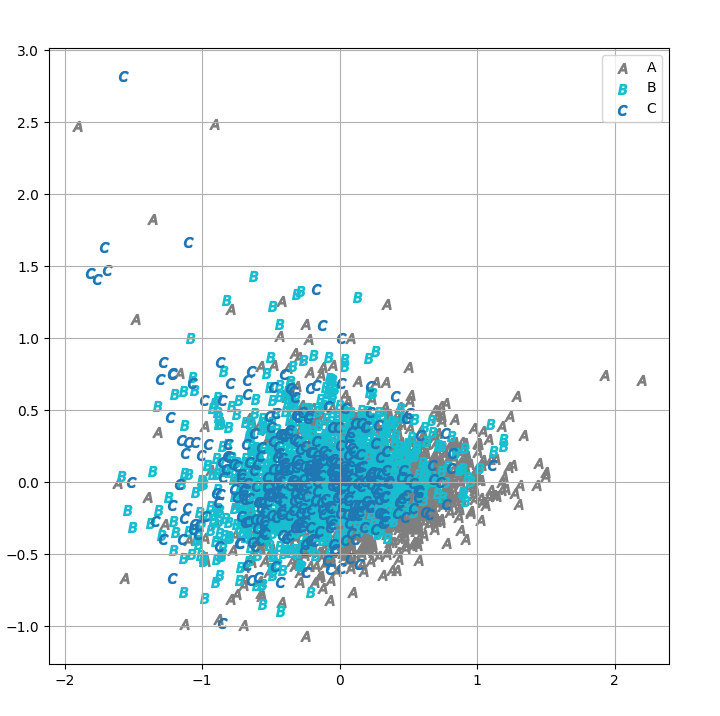
\includegraphics[width=1\linewidth]{pca-surface.png}
   \caption{Surface features.}
\end{subfigure}%
\begin{subfigure}{0.5\textwidth}
  \centering
  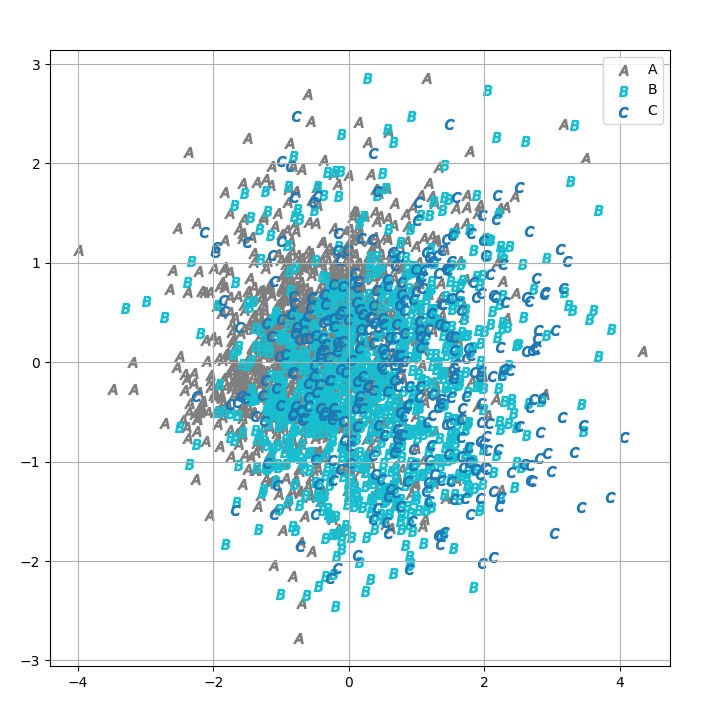
\includegraphics[width=1\linewidth]{pca-lexical.png}
  \caption{Lexical features.}
\end{subfigure}%

\begin{subfigure}{0.5\textwidth}
  \centering
  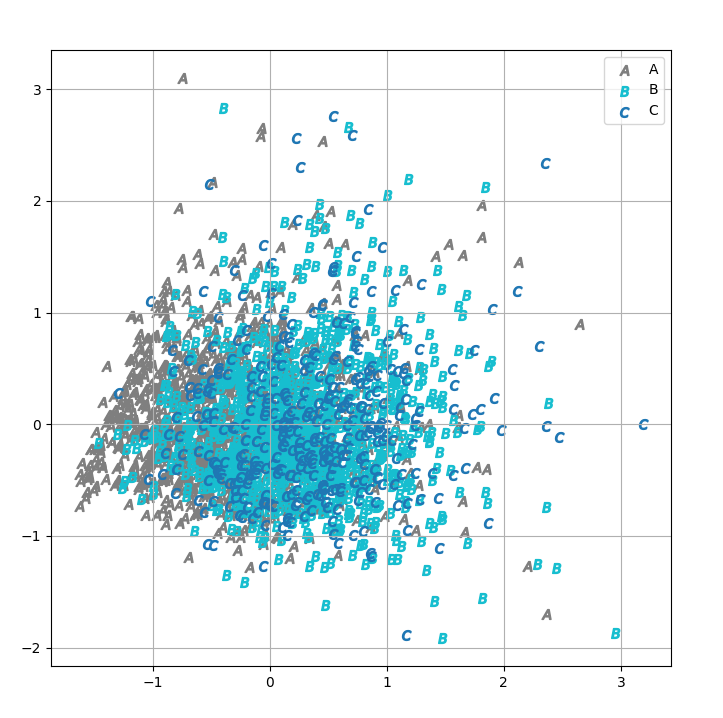
\includegraphics[width=1\linewidth]{pca-msy.png}
  \caption{Morphosyntactic features.}
\end{subfigure}%
\begin{subfigure}{0.5\textwidth}
  \centering
  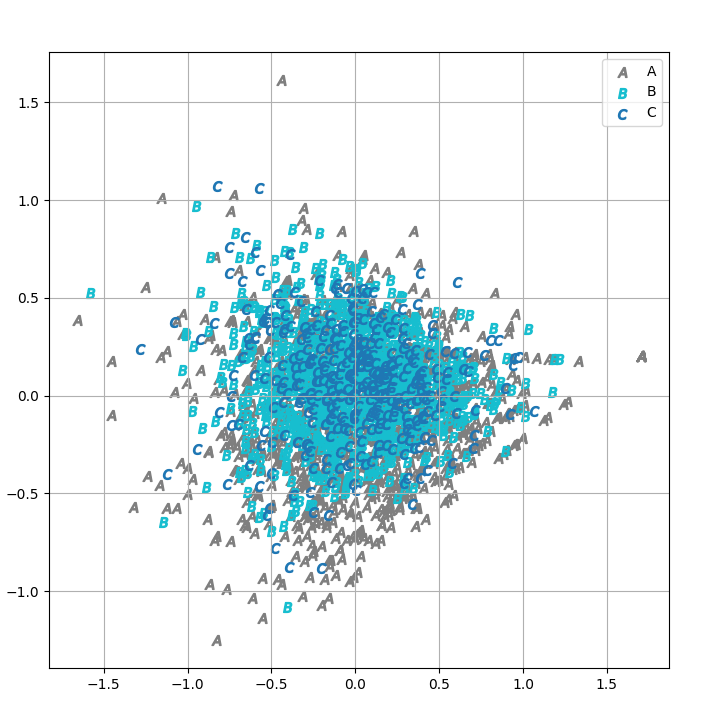
\includegraphics[width=1\textwidth]{pca-coh.png}
  \caption{Cohesion features.}
\end{subfigure}
\caption{Principal component analysis for different feature subsets.}
\label{fig:pca-sub}
\end{figure}


\begin{figure}[H]
    \centering
    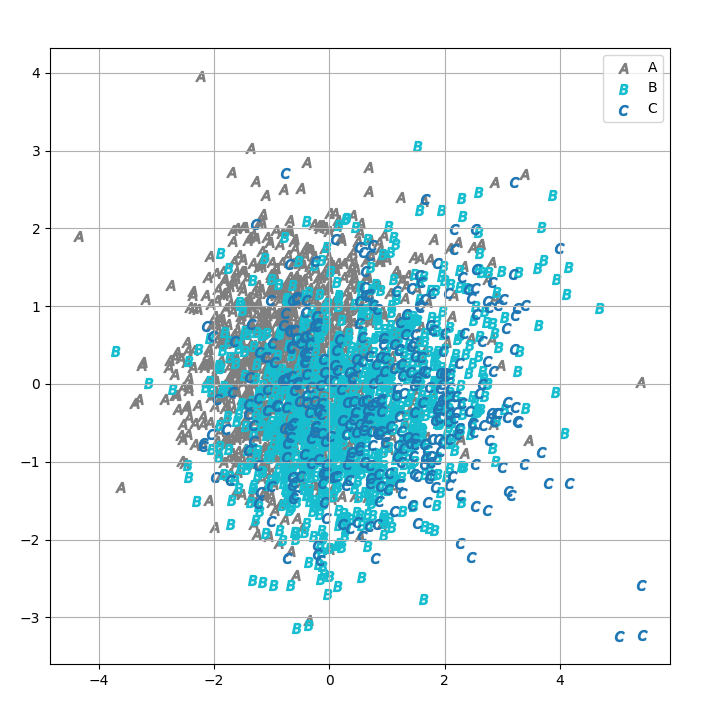
\includegraphics[width=1\linewidth]{images/pca-all.png}
    \caption{Principal component analysis for combined features.}
    \label{fig:pca-all}
\end{figure}


\pagebreak

\section{Conclusion}

This thesis has presented the first purely linguistic complexity analysis for the automatic proficiency classification of {\scshape l2} Portuguese. Until recently, Portuguese had been largely neglected in this space, though its prominence as a global language calls for its inclusion. A large and diverse set of complexity features were compiled, with several global, lexical, morphosyntactic, and discursive features demonstrating good predictive ability, corroborating the assertions of similar analyses for other languages. This thesis has shown that complexity features can indeed be leveraged to classify proficiency, though other metrics including part-of-speech \textit{n}-grams, errors, and task information may be combined for better results. In addition, resources fine-tuned for Portuguese learner text will likely improve accuracy even further.

\pagebreak

%%%%%%%%%%%%%%%%%%%%%%%%%%%%%%%%%%%% back matter

\bibliography{peripheral/bibliography.bib}

\end{document}